\documentclass[journal,12pt,twocolumn]{IEEEtran}

\usepackage{setspace}
\usepackage{gensymb}
\singlespacing
\usepackage[cmex10]{amsmath}

\usepackage{amsthm}

\usepackage{mathrsfs}
\usepackage{txfonts}
\usepackage{stfloats}
\usepackage{bm}
\usepackage{cite}
\usepackage{cases}
\usepackage{subfig}

\usepackage{longtable}
\usepackage{multirow}

\usepackage{enumitem}
\usepackage{mathtools}
\usepackage{steinmetz}
\usepackage{tikz}
\usepackage{circuitikz}
\usepackage{verbatim}
\usepackage{tfrupee}
\usepackage[breaklinks=true]{hyperref}
\usepackage{graphicx}
\usepackage{tkz-euclide}

\usetikzlibrary{calc,math}
\usepackage{listings}
    \usepackage{color}                                            %%
    \usepackage{array}                                            %%
    \usepackage{longtable}                                        %%
    \usepackage{calc}                                             %%
    \usepackage{multirow}                                         %%
    \usepackage{hhline}                                           %%
    \usepackage{ifthen}                                           %%
    \usepackage{lscape}     
\usepackage{multicol}
\usepackage{chngcntr}

\DeclareMathOperator*{\Res}{Res}

\renewcommand\thesection{\arabic{section}}
\renewcommand\thesubsection{\thesection.\arabic{subsection}}
\renewcommand\thesubsubsection{\thesubsection.\arabic{subsubsection}}

\renewcommand\thesectiondis{\arabic{section}}
\renewcommand\thesubsectiondis{\thesectiondis.\arabic{subsection}}
\renewcommand\thesubsubsectiondis{\thesubsectiondis.\arabic{subsubsection}}


\hyphenation{op-tical net-works semi-conduc-tor}
\def\inputGnumericTable{}                                 %%

\lstset{
%language=C,
frame=single, 
breaklines=true,
columns=fullflexible
}
\begin{document}


\newtheorem{theorem}{Theorem}[section]
\newtheorem{problem}{Problem}
\newtheorem{proposition}{Proposition}[section]
\newtheorem{lemma}{Lemma}[section]
\newtheorem{corollary}[theorem]{Corollary}
\newtheorem{example}{Example}[section]
\newtheorem{definition}[problem]{Definition}

\newcommand{\BEQA}{\begin{eqnarray}}
\newcommand{\EEQA}{\end{eqnarray}}
\newcommand{\define}{\stackrel{\triangle}{=}}
\bibliographystyle{IEEEtran}
\raggedbottom
\setlength{\parindent}{0pt}
\providecommand{\mbf}{\mathbf}
\providecommand{\pr}[1]{\ensuremath{\Pr\left(#1\right)}}
\providecommand{\qfunc}[1]{\ensuremath{Q\left(#1\right)}}
\providecommand{\sbrak}[1]{\ensuremath{{}\left[#1\right]}}
\providecommand{\lsbrak}[1]{\ensuremath{{}\left[#1\right.}}
\providecommand{\rsbrak}[1]{\ensuremath{{}\left.#1\right]}}
\providecommand{\brak}[1]{\ensuremath{\left(#1\right)}}
\providecommand{\lbrak}[1]{\ensuremath{\left(#1\right.}}
\providecommand{\rbrak}[1]{\ensuremath{\left.#1\right)}}
\providecommand{\cbrak}[1]{\ensuremath{\left\{#1\right\}}}
\providecommand{\lcbrak}[1]{\ensuremath{\left\{#1\right.}}
\providecommand{\rcbrak}[1]{\ensuremath{\left.#1\right\}}}
\theoremstyle{remark}
\newtheorem{rem}{Remark}
\newcommand{\sgn}{\mathop{\mathrm{sgn}}}
% \providecommand{\abs}[1]{\left\vert#1\right\vert}
% \providecommand{\res}[1]{\Res\displaylimits_{#1}} 
% \providecommand{\norm}[1]{\left\lVert#1\right\rVert}
% %\providecommand{\norm}[1]{\lVert#1\rVert}
% \providecommand{\mtx}[1]{\mathbf{#1}}
% \providecommand{\mean}[1]{E\left[ #1 \right]}
\providecommand{\fourier}{\overset{\mathcal{F}}{ \rightleftharpoons}}
%\providecommand{\hilbert}{\overset{\mathcal{H}}{ \rightleftharpoons}}
\providecommand{\system}{\overset{\mathcal{H}}{ \longleftrightarrow}}
	%\newcommand{\solution}[2]{\textbf{Solution:}{#1}}
\newcommand{\solution}{\noindent \textbf{Solution: }}
\newcommand{\cosec}{\,\text{cosec}\,}
\providecommand{\dec}[2]{\ensuremath{\overset{#1}{\underset{#2}{\gtrless}}}}
\newcommand{\myvec}[1]{\ensuremath{\begin{pmatrix}#1\end{pmatrix}}}
\newcommand{\mydet}[1]{\ensuremath{\begin{vmatrix}#1\end{vmatrix}}}
\numberwithin{equation}{subsection}
\makeatletter
\@addtoreset{figure}{problem}
\makeatother
\let\StandardTheFigure\thefigure
\let\vec\mathbf
\renewcommand{\thefigure}{\theproblem}
\def\putbox#1#2#3{\makebox[0in][l]{\makebox[#1][l]{}\raisebox{\baselineskip}[0in][0in]{\raisebox{#2}[0in][0in]{#3}}}}
     \def\rightbox#1{\makebox[0in][r]{#1}}
     \def\centbox#1{\makebox[0in]{#1}}
     \def\topbox#1{\raisebox{-\baselineskip}[0in][0in]{#1}}
     \def\midbox#1{\raisebox{-0.5\baselineskip}[0in][0in]{#1}}
\vspace{3cm}
\title{Assignment 1}
\author{Varun SM - EE18BTECH11030}
\maketitle
\newpage
\bigskip
\renewcommand{\thefigure}{\theenumi}
\renewcommand{\thetable}{\theenumi}
Download all files from 
%
\begin{lstlisting}
https://github.com/Elonian/C_and_DataStructures/tree/main/Assignment_1
\end{lstlisting}
\section{Problem}
(Q 17) The following C program is executed on a Unix/Linux system
\begin{lstlisting}
#include <unistd.h>
int main(){
    int i;
    for(i = 0; i < 10; i++){
        if(i%2 == 0){
            fork();
        }
    }
}
\end{lstlisting}
The total number of child processes created are.

\section{Solution}
Answer: 
Number of child process created are ${2^{n}}$-1 = ${2^{5}}$-1 = 31.
Where n is the number of times fork() call occurred.
\newline
Explanation:
\begin{itemize}
    \item \textbf{fork()} is used for process creation on Unix-like operating systems. It wont take any arguments and returns process ID. 
    \item The purpose of fork() is to create a new process, which becomes the child process of the caller(Parent process).
    \item After a new child process is created, both processes will execute the next instruction following the fork() system call.
\end{itemize}

In the \textbf{for} loop \textbf{if} condition is satisfied only for even values of i;

First fork method is called at i = 0 and child process is created with variable i = 0 in child process (c1).

In level 1 one child process(c1) and parent process(p) is running.
 
In parent process(p) when i = 2 . it calls fork method then a new child process(c2) is created with variable i = 2.

similarly for the child process(c1) at i = 2 another child process(c3) is created.

At each level in row all the child processes along with parent process running at given instant are present.

In the Level 2 total number of child process = 3 = ${2^L}$ -1.

where L is the highest level of tree or number of times fork() call occurred.

This process creation continuous till level 5 because variable \textbf{i} takes even values.

Number of child process at level 5 = ${2^5}$ -1 = 31.


Graphically it is depicted as below.

\begin{figure}[!h]
\centering
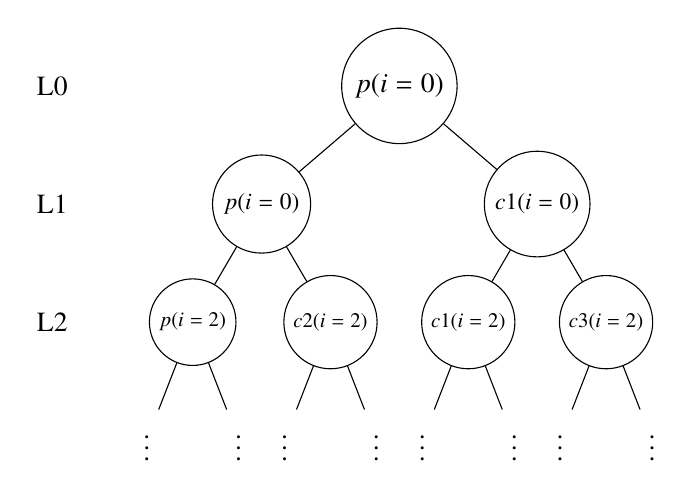
\begin{tikzpicture}[level/.style={sibling distance=35mm/#1}]
\node [circle,draw,scale=1] (z){$p(i=0)$}
  child {node [circle,draw,scale=0.85] (a) {$p(i=0)$}
    child {node [circle,draw,scale=0.75] (b) {$p(i=2)$}
      child {node {$\vdots$}
      child [grow=left, xshift=0.3cm] {node (r) {} edge from parent[draw=none]
      child [grow=up] {node (s) {L2} edge from parent[draw=none]
      child [grow=up] {node (t) {L1} edge from parent[draw=none]
      child [grow=up] {node (t) {L0} edge from parent[draw=none]}}}}
      } 
      child {node {$\vdots$}}
    }
     child {node [circle,draw,scale=0.75] (m) {$c2(i=2)$}
      child {node {$\vdots$}}
      child {node {$\vdots$}}
    }
  }
  child {node [circle,draw,scale=0.85] (j) {$c1(i=0)$}
    child {node [circle,draw,scale=0.75] (k) {$c1(i=2)$}
      child {node {$\vdots$}}
      child {node {$\vdots$}}
    }
  child {node [circle,draw,scale=0.75] (l) {$c3(i=2)$}
    child {node {$\vdots$}}
    child {node (c){$\vdots$}
    }
  }
};

\end{tikzpicture}
\caption{Tree representation} \label{fig:tree1}
\end{figure}

\end{document}

